\documentclass[12pt]{article}
\usepackage[utf8]{inputenc}
\usepackage{array}
\usepackage{xcolor}
\usepackage{graphicx}
\usepackage{mathtools}
\usepackage{amsmath}
\usepackage{multicol}
\usepackage{eqnarray}
\usepackage{wrapfig}


\usepackage{natbib}
\usepackage{hyperref}
\hypersetup{
	colorlinks=true,
	linkcolor=black,
	filecolor=mangeta,      
	urlcolor=blue,
	pdftitle={Overleaf Example},
	pdfpagemode=FullScreen,
}

\usepackage[margin=0.6in]{geometry}

\title{52nd—24th INTERNATIONAL-RUDOLF ORTVAY \\ PROBLEM SOLVING CONTEST IN PHYSICS \\ Problem 1}
\author{Nguyen Thanh Long}
\date{\today}

\begin{document}
	
\maketitle
	
\noindent We note the graph of a semi-cycloid-shaped can be performed by only one degree of freedom $\theta$:
\begin{align*}
	x & = R \left( 2 \theta - \sin 2 \theta \right) \\
	y & = R \left( 1 + \cos 2 \theta \right).
\end{align*}

\begin{center}
	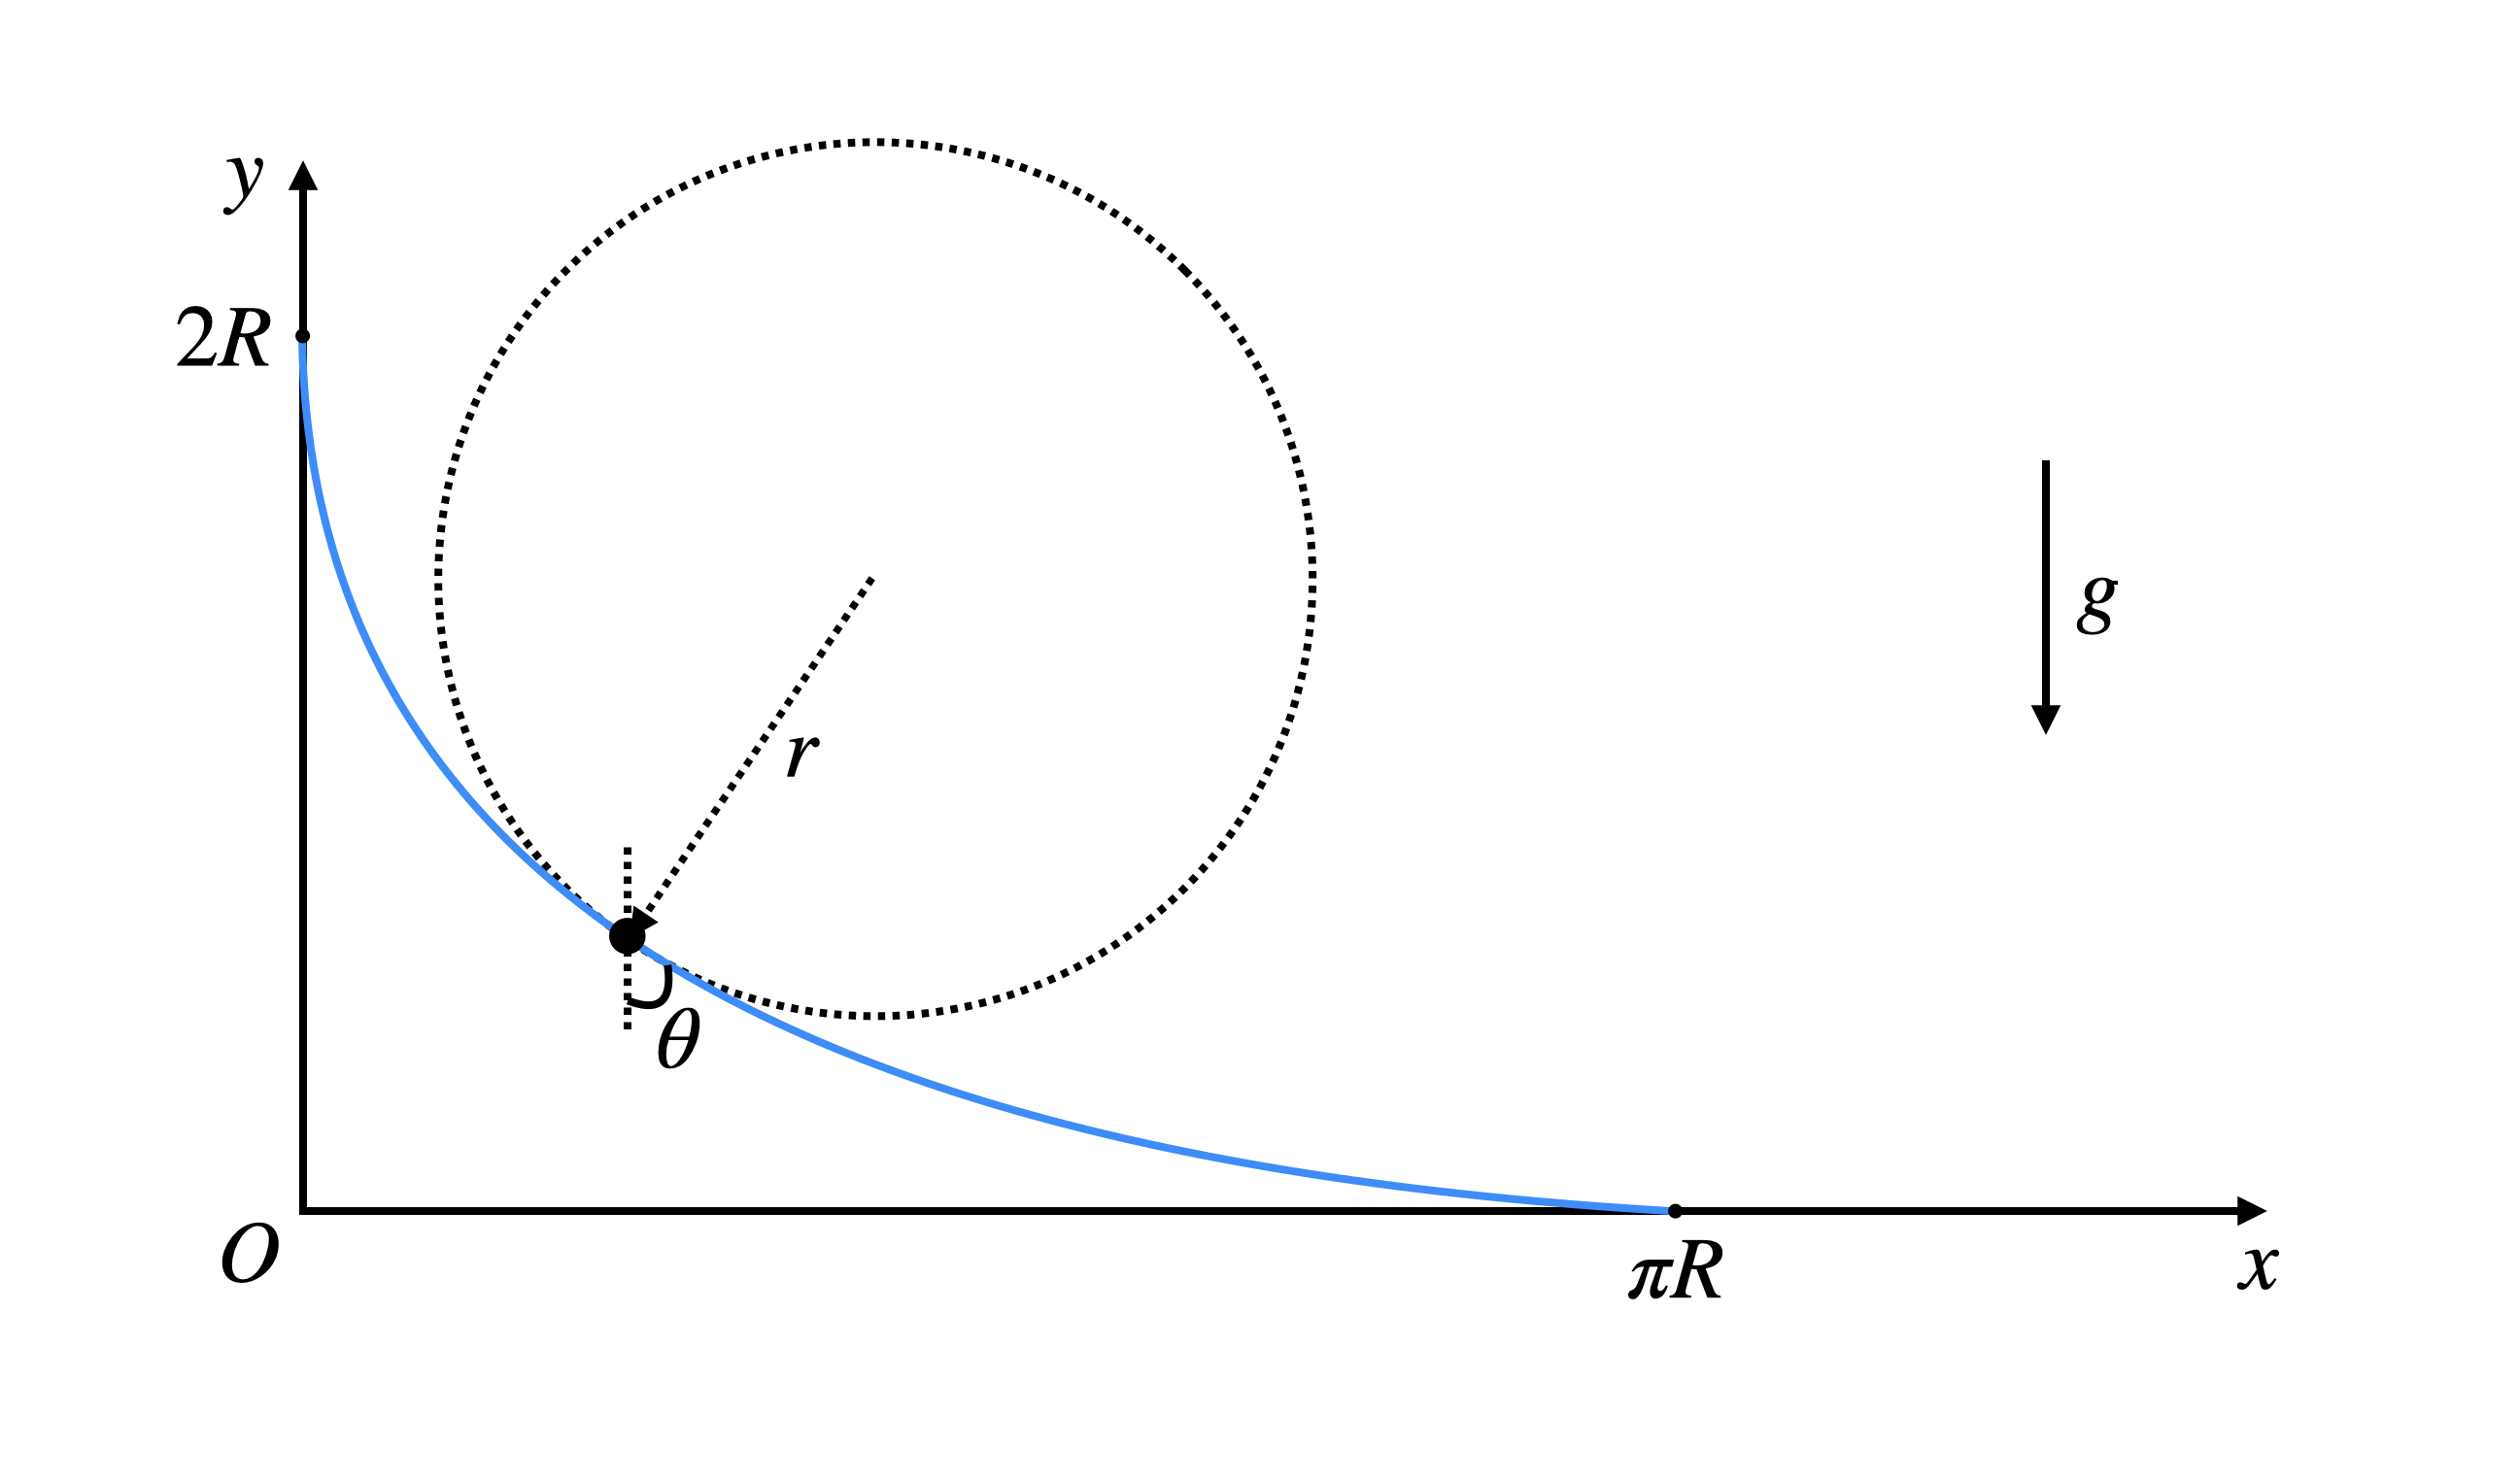
\includegraphics[width=0.8\textwidth]{Fig P1.png}
\end{center}	

\noindent We take differential of these equation and receive some result about this graph:
\begin{itemize}
	\item Angle formed by the tangent of the graph to the vertical is $\theta$.
	\item Radius of curvature:
	\begin{align*}
		r(\theta) & = \left| \frac{ \left[ x'(\theta)^2 + y'(\theta)^2 \right]^{\frac{3}{2}}}{x'(\theta) y"(\theta) - y'(\theta) x"(\theta)} \right| \\
		& = 4 R \sin \left( \theta \right) . 
	\end{align*}
    \item The speed of the body:
    \begin{align*}
    	v & = \sqrt{ \left( \frac{dx}{dt} \right)^2 + \left( \frac{dy}{dt} \right)^2 } \\
    	& = 4 R \sin \left( \theta \right) \dot{\theta} \\
    	\Rightarrow \dot{v} & = 4 R \cos \left( \theta \right) \dot{\theta}^2 + 4 R \sin \left( \theta \right) \ddot{\theta} .
    \end{align*}	
\end{itemize}	

\noindent When the body slides down the slope, $\theta$ run from $0$ (i.e $x=0$, $y= 2 R$) to $\frac{\pi}{2}$ (i.e $x= \pi R$, $y=0$).

\noindent The differential equation governing the motion of the body is:
\begin{itemize}
	\item Perpendicular to the orbital tangent: $\frac{m v^2}{r} = N - mg \sin \theta .$
	\item Orbital tangen: $ m \dot{v} = mg \cos \theta - \mu N.$
\end{itemize}	
$$\Rightarrow \dot{v} = g \left( \cos \theta - \mu \sin \theta \right) - \mu \frac{v^2}{r} .$$

\noindent Put $\dot{v}$, $v$, $\alpha$ and $r$ in this equation, we have:
$$ \ddot{\theta} + \left( \cot \theta - \mu \right) \dot{\theta}^2 = \frac{g}{4R} \left( \cot \theta - \mu \right) . $$
\noindent Multiply this equation with $ \sin^2 (\theta) e^{-2 \mu \theta}$:
\begin{align*}
	\frac{d}{d \theta} \left[ \dot{\theta}^2 \sin^2 (\theta) e^{-2 \mu \theta} \right] & = \frac{g}{2R} \left( \cot \theta - \mu \right) \sin^2 (\theta) e^{- 2 \mu \theta}. \\
	\Rightarrow \dot{\theta}^2 \sin^2 (\theta) e^{-2 \mu \theta} & = \frac{g}{4R} \sin^2 (x) e^{-2 \mu \theta} +C \\
	\Rightarrow \dot{\theta} & = \sqrt{ \frac{g}{4R} + \frac{C e^{2 \mu \theta}}{\sin^2 (\theta)}}
\end{align*}

\noindent At the bottom of slope ($\theta = \frac{\pi}{2}$), the body is stop (i.e $\dot{\theta} =0$), so we can find the constant $C = - \frac{g e^{-\mu \pi}}{4R}$. \\

\noindent Because when we choose the top of slope is the place to slide the body down, we can't receive a meaningful result, so we will choose a very close place with $\theta=\theta_0$  (with $\theta_0 \ll 1$) to solve this problem. Thus, we find $\mu$ to the body stop at the bottom of slope is:
$$ \mu = - \frac{2 \ln \left( \theta_0 \right) }{\pi} . $$


\end{document}